\section{Implementation} \label{sec:implementation}
We implemented the algorithm presented in this work, i.e.\ Algorithm~\ref{alg:bkw}, to verify the assumptions made in this work and to confirm the expected behaviour of the algorithm. Our implementation supports machine size ring elements and integer values for $b$. We mention that our implementation is not optimised and hence we do not report CPU times. \anonymous{Our implementation is available through the programme chair.}{Our implementation is available at \url{http://bitbucket.org/malb/bkw-lwe}.}

\subsection{Independence Assumption}\label{ss:independence}
To verify the independence assumption, i.e.\ Assumption~\ref{ass:independence}, and in particular that the noise part behaves like discrete Gaussian modulo $q$ with $s = \sqrt{2^a}\alpha q$, we ran our implementation for $q=4093,\sigma=3.0$, and $b=2$ with $n=10$, $25$ and $30$. In each case, we asked for $2^{20}$ samples and extracted the noise by computing $c_i - \dotp{\shortvec{a}_i}{\vec{s}}$ and analysed the resulting distributions. In all our experiments, the noise followed a discrete Gaussian closely. In Figure~\ref{fig:noise-n30} we plot a histogram for the experimental data (in gray) for the case $n=30$ and the expected distribution for $\mathcal{N}(0,\sqrt{2^a}q)$.

\begin{figure}
\begin{center}
 \begin{tikzpicture}
\pgfplotsset{width=0.7\textwidth, height=0.4\textwidth}
\begin{axis}[xlabel={$x$},ylabel={\# samples},ymin=0]

\addplot[smooth,mark=,gray,fill=gray,opacity=0.5,thick] table[x index=0,y index=1, col sep=comma] {noise-4093-30-2-3-20.dat};
\addlegendentry{observed data}

\addplot[smooth,mark=,black] table[x index=2,y index=3, col sep=comma] {noise-4093-30-2-3-20.dat};
\addlegendentry{$\mathcal{N}(0,\sqrt{2^a}\alpha q)$}
\end{axis}
\end{tikzpicture}
\caption{Distribution of $c_i - \dotp{\shortvec{a}_i}{\vec{s}}$ for parameters $q=4093, n=30, a=15,\sigma = 3.0$.}
\label{fig:noise-n30}
\end{center}
\end{figure}


\subsection{Correctness of Algorithm~\ref{alg:variance}}

The behaviour our algorithm depends critically on the quality of approximation made in Algorithm~\ref{alg:variance}. We hence verified that the matrix $\vec{M}$ returned by that algorithm matches the actual variances observed in practice.

We start, with an example where the prediction is quite precise. We considered the parameters $q=65521$, $a=20$, $b=2$, $p = 2^{11}$ and $o = 2^{26}$. Algorithm~\ref{alg:variance} returns the following matrix 

\begin{footnotesize}
\begin{eqnarray*}
\log_2 \vec{M} &=& \left(\begin{array}{cccccccccccccccccccc} 
 28.4 & 28.4 & 28.4 & 28.4 & 28.4 & 28.4 & 28.4 & 28.4 & 28.4 & 28.4 & 28.4 & 28.4 & 28.4 & 28.4 & 28.4 & 28.4 & 28.4 & 28.4 & 28.4 & 28.4\\
  6.6 & 28.4 & 28.4 & 28.4 & 28.4 & 28.4 & 28.4 & 28.4 & 28.4 & 28.4 & 28.4 & 28.4 & 28.4 & 28.4 & 28.4 & 28.4 & 28.4 & 28.4 & 28.4 & 28.4\\
  7.7 &  7.0 & 28.4 & 28.4 & 28.4 & 28.4 & 28.4 & 28.4 & 28.4 & 28.4 & 28.4 & 28.4 & 28.4 & 28.4 & 28.4 & 28.4 & 28.4 & 28.4 & 28.4 & 28.4\\
  8.6 &  7.9 &  7.1 & 28.4 & 28.4 & 28.4 & 28.4 & 28.4 & 28.4 & 28.4 & 28.4 & 28.4 & 28.4 & 28.4 & 28.4 & 28.4 & 28.4 & 28.4 & 28.4 & 28.4\\
  9.5 &  8.9 &  8.1 &  7.2 & 28.4 & 28.4 & 28.4 & 28.4 & 28.4 & 28.4 & 28.4 & 28.4 & 28.4 & 28.4 & 28.4 & 28.4 & 28.4 & 28.4 & 28.4 & 28.4\\
 10.5 &  9.8 &  9.0 &  8.1 &  7.2 & 28.4 & 28.4 & 28.4 & 28.4 & 28.4 & 28.4 & 28.4 & 28.4 & 28.4 & 28.4 & 28.4 & 28.4 & 28.4 & 28.4 & 28.4\\
 11.4 & 10.8 & 10.0 &  9.1 &  8.2 &  7.3 & 28.4 & 28.4 & 28.4 & 28.4 & 28.4 & 28.4 & 28.4 & 28.4 & 28.4 & 28.4 & 28.4 & 28.4 & 28.4 & 28.4\\
 12.4 & 11.7 & 10.9 & 10.0 &  9.1 &  8.2 &  7.3 & 28.4 & 28.4 & 28.4 & 28.4 & 28.4 & 28.4 & 28.4 & 28.4 & 28.4 & 28.4 & 28.4 & 28.4 & 28.4\\
 13.3 & 12.7 & 11.9 & 11.0 & 10.1 &  9.2 &  8.2 &  7.3 & 28.4 & 28.4 & 28.4 & 28.4 & 28.4 & 28.4 & 28.4 & 28.4 & 28.4 & 28.4 & 28.4 & 28.4\\
 14.3 & 13.6 & 12.8 & 11.9 & 11.1 & 10.1 &  9.2 &  8.3 &  7.3 & 28.4 & 28.4 & 28.4 & 28.4 & 28.4 & 28.4 & 28.4 & 28.4 & 28.4 & 28.4 & 28.4\\
 15.3 & 14.6 & 13.8 & 12.9 & 12.0 & 11.1 & 10.2 &  9.2 &  8.3 &  7.3 & 28.4 & 28.4 & 28.4 & 28.4 & 28.4 & 28.4 & 28.4 & 28.4 & 28.4 & 28.4\\
 16.2 & 15.6 & 14.7 & 13.9 & 13.0 & 12.1 & 11.1 & 10.2 &  9.2 &  8.3 &  7.3 & 28.4 & 28.4 & 28.4 & 28.4 & 28.4 & 28.4 & 28.4 & 28.4 & 28.4\\
 17.2 & 16.5 & 15.7 & 14.8 & 13.9 & 13.0 & 12.1 & 11.2 & 10.2 &  9.3 &  8.3 &  7.3 & 28.4 & 28.4 & 28.4 & 28.4 & 28.4 & 28.4 & 28.4 & 28.4\\
 18.2 & 17.5 & 16.7 & 15.8 & 14.9 & 14.0 & 13.1 & 12.1 & 11.2 & 10.2 &  9.3 &  8.3 &  7.3 & 28.4 & 28.4 & 28.4 & 28.4 & 28.4 & 28.4 & 28.4\\
 19.1 & 18.5 & 17.7 & 16.8 & 15.9 & 15.0 & 14.0 & 13.1 & 12.2 & 11.2 & 10.2 &  9.3 &  8.3 &  7.4 & 28.4 & 28.4 & 28.4 & 28.4 & 28.4 & 28.4\\
 20.1 & 19.4 & 18.6 & 17.8 & 16.9 & 15.9 & 15.0 & 14.1 & 13.1 & 12.2 & 11.2 & 10.3 &  9.3 &  8.3 &  7.4 & 28.4 & 28.4 & 28.4 & 28.4 & 28.4\\
 21.1 & 20.4 & 19.6 & 18.7 & 17.8 & 16.9 & 16.0 & 15.0 & 14.1 & 13.1 & 12.2 & 11.2 & 10.3 &  9.3 &  8.3 &  7.4 & 28.4 & 28.4 & 28.4 & 28.4\\
 22.1 & 21.4 & 20.6 & 19.7 & 18.8 & 17.9 & 17.0 & 16.0 & 15.1 & 14.1 & 13.2 & 12.2 & 11.2 & 10.3 &  9.3 &  8.3 &  7.4 & 28.4 & 28.4 & 28.4\\
 23.0 & 22.4 & 21.6 & 20.7 & 19.8 & 18.9 & 17.9 & 17.0 & 16.1 & 15.1 & 14.1 & 13.2 & 12.2 & 11.3 & 10.3 &  9.3 &  8.3 &  7.4 & 28.4 & 28.4\\
 24.0 & 23.3 & 22.5 & 21.7 & 20.8 & 19.9 & 18.9 & 18.0 & 17.0 & 16.1 & 15.1 & 14.2 & 13.2 & 12.2 & 11.3 & 10.3 &  9.3 &  8.3 &  7.4 & 28.4\\
\end{array}\right)
\end{eqnarray*}
\end{footnotesize}

whereas our implementation constructed tables with the follow variance matrix

\begin{footnotesize}
\begin{eqnarray*}
\log_2 \vec{M}' &=& \left(\begin{array}{cccccccccccccccccccc} 
28.4 & 28.4 & 28.4 & 28.4 & 28.4 & 28.4 & 28.4 & 28.4 & 28.4 & 28.4 & 28.4 & 28.4 & 28.4 & 28.4 & 28.4 & 28.4 & 28.4 & 28.4 & 28.4 & 28.4\\
 6.6 & 28.4 & 28.4 & 28.4 & 28.4 & 28.4 & 28.4 & 28.4 & 28.4 & 28.4 & 28.4 & 28.4 & 28.4 & 28.4 & 28.4 & 28.4 & 28.4 & 28.4 & 28.4 & 28.4\\
 7.6 &  6.9 & 28.4 & 28.4 & 28.4 & 28.4 & 28.4 & 28.4 & 28.4 & 28.4 & 28.4 & 28.4 & 28.4 & 28.4 & 28.4 & 28.4 & 28.4 & 28.4 & 28.4 & 28.4\\
 8.5 &  7.8 &  7.1 & 28.4 & 28.4 & 28.4 & 28.4 & 28.4 & 28.4 & 28.4 & 28.4 & 28.4 & 28.4 & 28.4 & 28.4 & 28.4 & 28.4 & 28.4 & 28.4 & 28.4\\
 9.5 &  8.8 &  8.0 &  7.2 & 28.4 & 28.4 & 28.4 & 28.4 & 28.4 & 28.4 & 28.4 & 28.4 & 28.4 & 28.4 & 28.4 & 28.4 & 28.4 & 28.4 & 28.4 & 28.4\\
10.4 &  9.7 &  8.9 &  8.1 &  7.3 & 28.4 & 28.4 & 28.4 & 28.4 & 28.4 & 28.4 & 28.4 & 28.4 & 28.4 & 28.4 & 28.4 & 28.4 & 28.4 & 28.4 & 28.4\\
11.4 & 10.7 &  9.9 &  9.1 &  8.2 &  7.3 & 28.4 & 28.4 & 28.4 & 28.4 & 28.4 & 28.4 & 28.4 & 28.4 & 28.4 & 28.4 & 28.4 & 28.4 & 28.4 & 28.4\\
12.4 & 11.6 & 10.8 & 10.0 &  9.2 &  8.3 &  7.3 & 28.4 & 28.4 & 28.4 & 28.4 & 28.4 & 28.4 & 28.4 & 28.4 & 28.4 & 28.4 & 28.4 & 28.4 & 28.4\\
13.3 & 12.6 & 11.8 & 11.0 & 10.1 &  9.2 &  8.3 &  7.4 & 28.4 & 28.4 & 28.4 & 28.4 & 28.4 & 28.4 & 28.4 & 28.4 & 28.4 & 28.4 & 28.4 & 28.4\\
14.3 & 13.6 & 12.8 & 12.0 & 11.1 & 10.2 &  9.3 &  8.3 &  7.4 & 28.4 & 28.4 & 28.4 & 28.4 & 28.4 & 28.4 & 28.4 & 28.4 & 28.4 & 28.4 & 28.4\\
15.3 & 14.5 & 13.8 & 12.9 & 12.1 & 11.2 & 10.3 &  9.3 &  8.4 &  7.4 & 28.4 & 28.4 & 28.4 & 28.4 & 28.4 & 28.4 & 28.4 & 28.4 & 28.4 & 28.4\\
16.3 & 15.5 & 14.7 & 13.9 & 13.1 & 12.2 & 11.3 & 10.3 &  9.4 &  8.4 &  7.4 & 28.4 & 28.4 & 28.4 & 28.4 & 28.4 & 28.4 & 28.4 & 28.4 & 28.4\\
17.3 & 16.5 & 15.7 & 14.9 & 14.0 & 13.2 & 12.2 & 11.3 & 10.3 &  9.4 &  8.4 &  7.4 & 28.4 & 28.4 & 28.4 & 28.4 & 28.4 & 28.4 & 28.4 & 28.4\\
18.3 & 17.5 & 16.7 & 15.9 & 15.0 & 14.1 & 13.2 & 12.3 & 11.3 & 10.4 &  9.4 &  8.4 &  7.4 & 28.4 & 28.4 & 28.4 & 28.4 & 28.4 & 28.4 & 28.4\\
19.3 & 18.5 & 17.7 & 16.9 & 16.0 & 15.1 & 14.2 & 13.3 & 12.3 & 11.4 & 10.4 &  9.4 &  8.4 &  7.4 & 28.4 & 28.4 & 28.4 & 28.4 & 28.4 & 28.4\\
20.3 & 19.5 & 18.7 & 17.9 & 17.0 & 16.1 & 15.2 & 14.3 & 13.3 & 12.4 & 11.4 & 10.4 &  9.4 &  8.4 &  7.4 & 28.4 & 28.4 & 28.4 & 28.4 & 28.4\\
21.3 & 20.5 & 19.7 & 18.9 & 18.0 & 17.1 & 16.2 & 15.3 & 14.3 & 13.4 & 12.4 & 11.4 & 10.4 &  9.4 &  8.4 &  7.4 & 28.4 & 28.4 & 28.4 & 28.4\\
22.2 & 21.5 & 20.7 & 19.8 & 19.0 & 18.1 & 17.2 & 16.3 & 15.3 & 14.3 & 13.4 & 12.4 & 11.4 & 10.4 &  9.4 &  8.4 &  7.4 & 28.4 & 28.4 & 28.4\\
23.2 & 22.4 & 21.7 & 20.8 & 20.0 & 19.1 & 18.2 & 17.3 & 16.3 & 15.3 & 14.4 & 13.4 & 12.4 & 11.4 & 10.4 &  9.4 &  8.4 &  7.4 & 28.4 & 28.4\\
24.2 & 23.4 & 22.6 & 21.8 & 21.0 & 20.1 & 19.2 & 18.2 & 17.3 & 16.3 & 15.4 & 14.4 & 13.4 & 12.4 & 11.4 & 10.4 &  9.4 &  8.4 &  7.4 & 28.4\\
\end{array}\right)
\end{eqnarray*}
\end{footnotesize}

To highlight the limitations of Algorithm~\ref{alg:variance} we consider the parameters $q=65521, n=30, b=3, \sigma = 1.0, p = 2^8$ and $o=2^{29}$. Algorithm~\ref{alg:variance} predicts

\begin{footnotesize}
\begin{eqnarray*}
\log_2 \vec{M}' &=& \left(\begin{array}{cccccccccc} 
28.4 & 28.4 & 28.4 & 28.4 & 28.4 & 28.4 & 28.4 & 28.4 & 28.4 & 28.4\\
11.8 & 28.4 & 28.4 & 28.4 & 28.4 & 28.4 & 28.4 & 28.4 & 28.4 & 28.4\\
12.9 & 12.5 & 28.4 & 28.4 & 28.4 & 28.4 & 28.4 & 28.4 & 28.4 & 28.4\\
13.8 & 13.4 & 12.8 & 28.4 & 28.4 & 28.4 & 28.4 & 28.4 & 28.4 & 28.4\\
14.6 & 14.2 & 13.6 & 12.9 & 28.4 & 28.4 & 28.4 & 28.4 & 28.4 & 28.4\\
15.5 & 15.1 & 14.5 & 13.8 & 13.0 & 28.4 & 28.4 & 28.4 & 28.4 & 28.4\\
16.3 & 15.9 & 15.3 & 14.6 & 13.9 & 13.1 & 28.4 & 28.4 & 28.4 & 28.4\\
17.2 & 16.8 & 16.2 & 15.5 & 14.8 & 13.9 & 13.1 & 28.4 & 28.4 & 28.4\\
18.1 & 17.7 & 17.1 & 16.4 & 15.6 & 14.8 & 14.0 & 13.1 & 28.4 & 28.4\\
19.0 & 18.6 & 18.0 & 17.3 & 16.5 & 15.7 & 14.9 & 14.0 & 13.2 & 28.4\\
\end{array}\right)
\end{eqnarray*}
\end{footnotesize}
but implementation produced tables with variance matrix
\begin{footnotesize}
\begin{eqnarray*}
\log_2 \vec{M} &=& \left(\begin{array}{cccccccccc} 
28.4 & 28.4 & 28.4 & 28.4 & 28.4 & 28.4 & 28.4 & 28.4 & 28.4 & 28.4\\
11.7 & 28.4 & 28.4 & 28.4 & 28.4 & 28.4 & 28.4 & 28.4 & 28.4 & 28.4\\
12.6 & 12.4 & 28.4 & 28.4 & 28.4 & 28.4 & 28.4 & 28.4 & 28.4 & 28.4\\
13.4 & 13.2 & 12.8 & 28.4 & 28.4 & 28.4 & 28.4 & 28.4 & 28.4 & 28.4\\
14.1 & 13.9 & 13.5 & 13.0 & 28.4 & 28.4 & 28.4 & 28.4 & 28.4 & 28.4\\
14.8 & 14.6 & 14.2 & 13.7 & 13.1 & 28.4 & 28.4 & 28.4 & 28.4 & 28.4\\
15.4 & 15.3 & 15.0 & 14.5 & 13.9 & 13.2 & 28.4 & 28.4 & 28.4 & 28.4\\
16.1 & 16.0 & 15.7 & 15.3 & 14.7 & 14.0 & 13.2 & 28.4 & 28.4 & 28.4\\
16.9 & 16.7 & 16.4 & 16.0 & 15.5 & 14.9 & 14.1 & 13.3 & 28.4 & 28.4\\
17.6 & 17.4 & 17.2 & 16.8 & 16.3 & 15.7 & 15.0 & 14.2 & 13.3 & 28.4\\
\end{array}\right)
\end{eqnarray*}
\end{footnotesize}
which means we overestimated the variance of child components in our tables $T$.

The main reason for this effect is that our approximation of the shrinking of variances when taking the minimum is based on the uniform distribution. However, the distributions actually governing the entries of our tables $T^\ell$ are not uniform, as discussed in \ref{sec:control-growth}. Figure~\ref{fig:table-dist} gives histograms for these distributions.

\begin{figure}
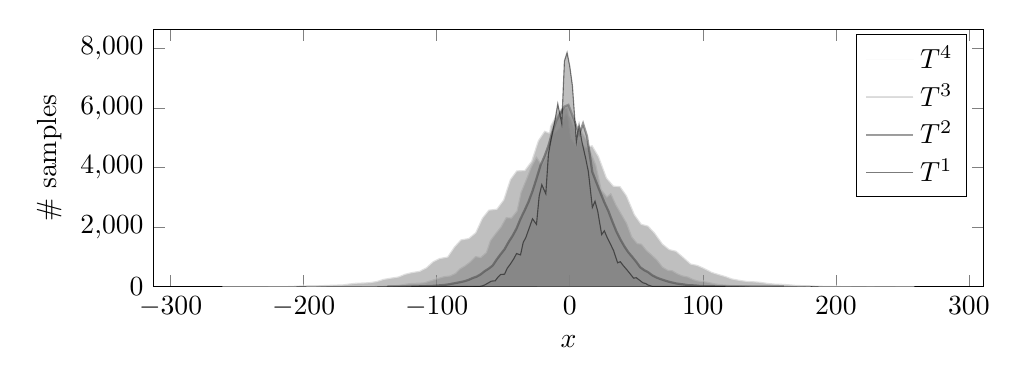
\begin{tikzpicture}
\pgfplotsset{width=1.0\textwidth, height=0.4\textwidth}
\begin{axis}[xlabel={$x$},ylabel={\# samples},ymin=0]

\addplot[white,thick,fill=gray,opacity=0.5] coordinates {
( -261,5.5)  ( -255,5.5)  ( -250,4.0)  ( -245,4.5)  ( -239,4.5)  ( -234,5.5)  ( -229,8.0)  ( -224,11.0)  ( -218,11.5)  ( -213,15.5)  ( -208,24.5)  ( -203,35.0)  ( -197,35.5)  ( -192,35.0)  ( -187,47.5)  ( -182,57.0)  ( -176,67.0)  ( -171,72.0)  ( -166,102.5)  ( -161,129.0)  ( -155,138.0)  ( -150,152.5)  ( -145,187.5)  ( -140,259.5)  ( -134,304.5)  ( -129,338.0)  ( -124,428.5)  ( -119,485.0)  ( -113,528.0)  ( -108,643.0)  ( -103,845.0)  (  -98,958.5)  (  -92,1008.5)  (  -87,1338.5)  (  -82,1584.5)  (  -76,1632.0)  (  -71,1819.0)  (  -66,2307.0)  (  -61,2585.5)  (  -55,2616.5)  (  -50,2918.5)  (  -45,3601.5)  (  -40,3905.5)  (  -34,3915.5)  (  -29,4218.0)  (  -24,4904.5)  (  -19,5242.5)  (  -13,5130.5)  (   -8,5317.0)  (   -3,5818.5)  (    1,5674.5)  (    7,4938.5)  (   12,4685.5)  (   17,4754.0)  (   22,4375.0)  (   28,3654.5)  (   33,3391.0)  (   38,3376.0)  (   43,3056.5)  (   49,2419.0)  (   54,2107.5)  (   59,2048.5)  (   64,1811.0)  (   70,1438.0)  (   75,1258.5)  (   80,1203.5)  (   85,1013.5)  (   91,774.5)  (   96,727.0)  (  101,628.5)  (  107,490.0)  (  112,420.5)  (  117,355.0)  (  122,273.5)  (  128,223.5)  (  133,192.0)  (  138,180.5)  (  143,162.0)  (  149,122.5)  (  154,101.5)  (  159,95.0)  (  164,81.0)  (  170,56.5)  (  175,49.5)  (  180,44.0)  (  185,32.5)  (  191,25.0)  (  196,23.5)  (  201,20.5)  (  206,15.5)  (  212,9.0)  (  217,6.0)  (  222,9.0)  (  227,11.5)  (  233,5.5)  (  238,1.5)  (  243,1.5)  (  248,1.5)  (  254,1.5)  (  259,1.0) 
 };
\addlegendentry{$T^4$}

\addplot[lightgray,thick,fill=gray,opacity=0.5] coordinates {
( -198,1.5)  ( -194,1.0)  ( -190,0.5)  ( -186,0.0)  ( -182,1.5)  ( -178,2.0)  ( -175,2.5)  ( -171,5.0)  ( -167,6.0)  ( -163,6.0)  ( -159,7.0)  ( -155,10.5)  ( -152,13.5)  ( -148,23.0)  ( -144,31.5)  ( -140,34.5)  ( -136,41.0)  ( -132,48.0)  ( -129,56.5)  ( -125,85.0)  ( -121,113.0)  ( -117,125.5)  ( -113,130.0)  ( -109,147.0)  ( -106,192.5)  ( -102,248.0)  (  -98,304.5)  (  -94,354.5)  (  -90,373.0)  (  -86,458.5)  (  -83,601.0)  (  -79,709.0)  (  -75,845.0)  (  -71,1026.5)  (  -67,995.5)  (  -63,1155.0)  (  -60,1551.5)  (  -56,1789.0)  (  -52,2012.5)  (  -48,2332.0)  (  -44,2322.0)  (  -40,2547.0)  (  -37,3168.0)  (  -33,3602.5)  (  -29,4053.5)  (  -25,4383.0)  (  -21,4109.5)  (  -17,4438.0)  (  -14,5377.5)  (  -10,5711.5)  (   -6,5959.0)  (   -2,5974.5)  (    1,4999.0)  (    5,4741.5)  (    8,5242.0)  (   12,4936.0)  (   16,4529.0)  (   20,4083.0)  (   24,3264.0)  (   28,3035.5)  (   31,3149.5)  (   35,2757.0)  (   39,2447.5)  (   43,2141.0)  (   47,1675.5)  (   51,1458.5)  (   54,1442.0)  (   58,1223.5)  (   62,1066.5)  (   66,894.0)  (   70,666.0)  (   74,560.0)  (   77,552.5)  (   81,445.0)  (   85,372.0)  (   89,337.0)  (   93,249.5)  (   97,200.0)  (  100,189.5)  (  104,159.5)  (  108,119.5)  (  112,88.0)  (  116,73.5)  (  120,57.5)  (  123,53.5)  (  127,47.5)  (  131,40.0)  (  135,30.5)  (  139,18.5)  (  143,17.5)  (  146,20.0)  (  150,12.0)  (  154,7.5)  (  158,6.0)  (  162,2.0)  (  166,2.0)  (  169,2.0)  (  173,0.5)  (  177,1.5)  (  181,3.0) 
 };
\addlegendentry{$T^3$}

\addplot[darkgray,thick,fill=gray,opacity=0.5] coordinates {
( -137,1.5)  ( -133,0.5)  ( -130,0.5)  ( -127,1.0)  ( -124,1.0)  ( -121,1.5)  ( -118,2.5)  ( -115,4.0)  ( -112,7.5)  ( -109,13.0)  ( -106,16.0)  ( -103,22.0)  ( -100,33.5)  (  -97,43.0)  (  -94,54.5)  (  -91,74.0)  (  -88,99.5)  (  -85,124.0)  (  -82,151.0)  (  -79,180.5)  (  -76,225.0)  (  -73,285.0)  (  -70,333.0)  (  -67,408.5)  (  -64,515.0)  (  -61,599.5)  (  -58,703.0)  (  -55,902.0)  (  -52,1083.0)  (  -49,1254.5)  (  -46,1494.0)  (  -43,1703.0)  (  -40,1951.0)  (  -37,2277.0)  (  -34,2552.5)  (  -31,2848.0)  (  -28,3208.5)  (  -25,3628.5)  (  -22,4067.5)  (  -19,4372.0)  (  -16,4737.0)  (  -13,5200.0)  (  -10,5574.5)  (   -7,5826.5)  (   -4,6049.5)  (   -1,6108.0)  (    1,5872.5)  (    4,5512.0)  (    7,5117.5)  (   10,5479.0)  (   13,5049.5)  (   17,3847.5)  (   20,3501.0)  (   23,3161.0)  (   26,2831.5)  (   29,2543.0)  (   32,2189.0)  (   35,1860.5)  (   38,1590.5)  (   41,1354.5)  (   44,1154.5)  (   47,996.0)  (   50,830.0)  (   53,646.0)  (   56,551.0)  (   59,480.0)  (   62,378.5)  (   65,307.5)  (   68,254.0)  (   71,211.0)  (   74,167.5)  (   77,134.5)  (   80,104.0)  (   83,85.5)  (   86,68.0)  (   89,47.0)  (   92,42.5)  (   95,32.5)  (   98,18.0)  (  101,13.0)  (  104,11.5)  (  107,8.0)  (  110,5.0)  (  113,2.5)  (  116,3.5)  (  119,2.5)  (  122,0.0)  (  125,0.0)  (  128,0.0)  (  131,0.0)  (  134,0.0)  (  137,0.0)  (  140,0.0)  (  143,0.0)  (  146,0.0)  (  149,0.0)  (  152,0.0)  (  155,0.0)  (  158,0.0)  (  161,0.5) 
 };
\addlegendentry{$T^2$}


\addplot[black,fill=gray,opacity=0.5] coordinates {
( -119,1.5)  ( -116,0.0)  ( -114,0.5)  ( -111,0.5)  ( -109,0.0)  ( -107,0.0)  ( -104,1.0)  ( -102,1.5)  (  -99,0.5)  (  -97,1.0)  (  -95,1.0)  (  -92,0.0)  (  -90,0.0)  (  -87,0.0)  (  -85,0.5)  (  -83,1.0)  (  -80,1.5)  (  -78,1.5)  (  -76,1.0)  (  -73,1.0)  (  -71,1.5)  (  -68,3.0)  (  -66,19.0)  (  -64,51.5)  (  -61,126.5)  (  -59,180.0)  (  -56,194.0)  (  -54,314.5)  (  -52,404.5)  (  -49,415.5)  (  -47,614.0)  (  -45,733.0)  (  -42,937.0)  (  -40,1109.5)  (  -37,1065.0)  (  -35,1479.5)  (  -33,1650.0)  (  -30,2025.5)  (  -28,2277.5)  (  -25,2090.0)  (  -23,3037.0)  (  -21,3423.0)  (  -18,3119.5)  (  -16,4460.5)  (  -14,4941.0)  (  -11,5613.5)  (   -9,6141.0)  (   -6,5475.0)  (   -4,7579.0)  (   -2,7863.5)  (    0,7406.5)  (    2,6750.5)  (    5,4869.0)  (    7,5442.0)  (    9,4898.5)  (   12,4303.5)  (   14,3860.5)  (   17,2661.0)  (   19,2866.5)  (   21,2538.0)  (   24,1747.5)  (   26,1873.0)  (   28,1662.0)  (   31,1390.0)  (   33,1204.0)  (   36,798.5)  (   38,834.5)  (   40,717.0)  (   43,560.0)  (   45,450.5)  (   48,281.5)  (   50,297.0)  (   52,229.0)  (   55,125.5)  (   57,103.0)  (   59,49.5)  (   62,5.5)  (   64,2.0)  (   67,2.5)  (   69,1.5)  (   71,0.5)  (   74,1.0)  (   76,1.0)  (   79,0.0)  (   81,0.0)  (   83,0.0)  (   86,0.5)  (   88,1.0)  (   90,0.5)  (   93,0.0)  (   95,0.0)  (   98,0.5)  (  100,1.5)  (  102,1.0)  (  105,0.0)  (  107,0.0)  (  110,0.5)  (  112,1.0)  (  114,1.0)  (  117,1.0) 
};
\addlegendentry{$T^1$}
\end{axis}
\end{tikzpicture}
\label{fig:table-dist}
\caption{Histogram of distribution of $0$th component in $T^\ell$ for $1 \leq \ell \leq 4$ with parameters $q=32003$, $b=2$, $p=2^9$, $n=10$, and $o=2^{20}$.}
\end{figure}

Overall, for the instances considered our estimates are pessimistic, which means we expect our algorithm to perform better in practice than predicted. A more refined model for its behaviour is hence a good topic for future work.
